\begin{equation}
\label{eq:inclusive}
	m_{jj} > 200 \,\textrm{GeV}\,,\qquad |\Delta y_{jj}| > 2\,.
\end{equation}


The figure is Fig.~\ref{fig:ratio2d_LO}.

% \subsection{Validity of the VBS approximation}\label{subsec:VBSapprox}


\begin{figure}[hbt]
\centering
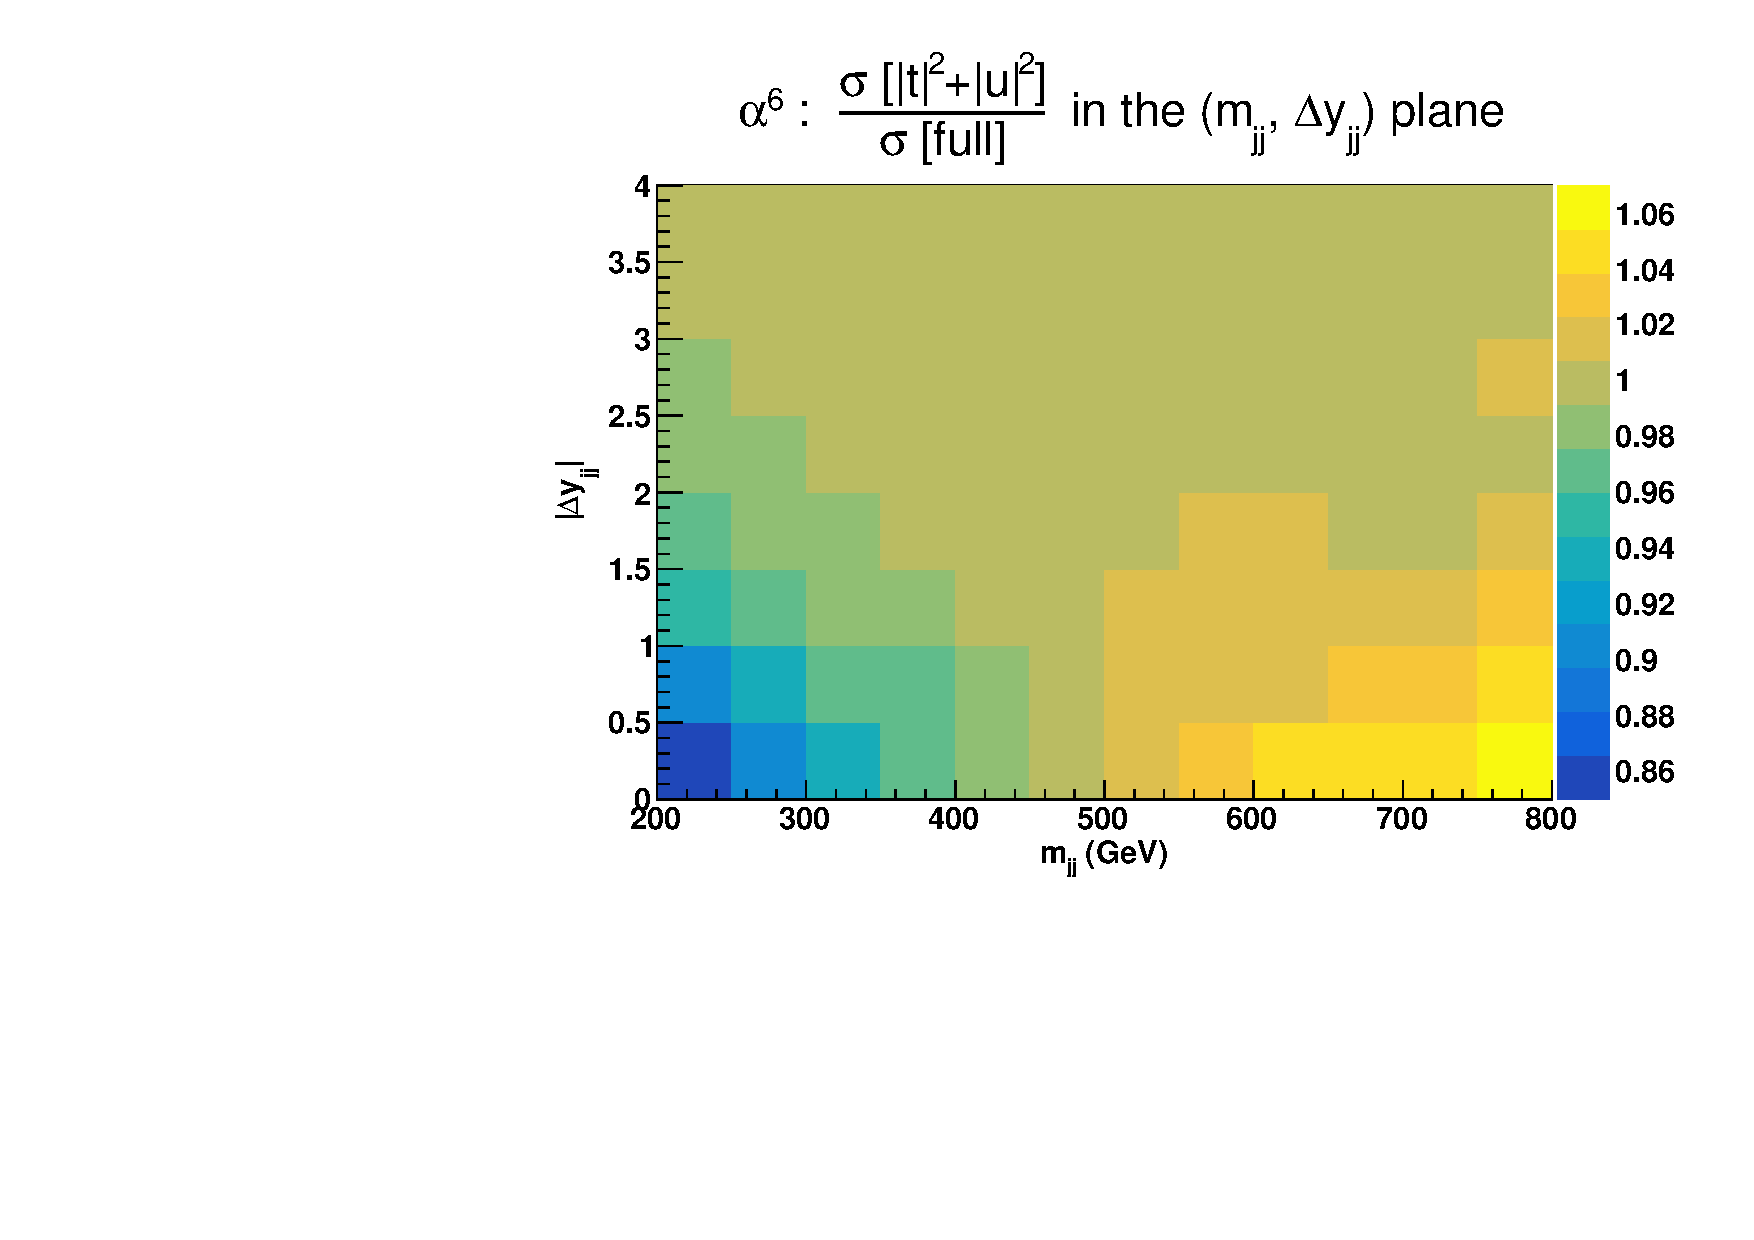
\includegraphics[scale=0.395]{figures/scanfigures/ratio_tu.pdf}
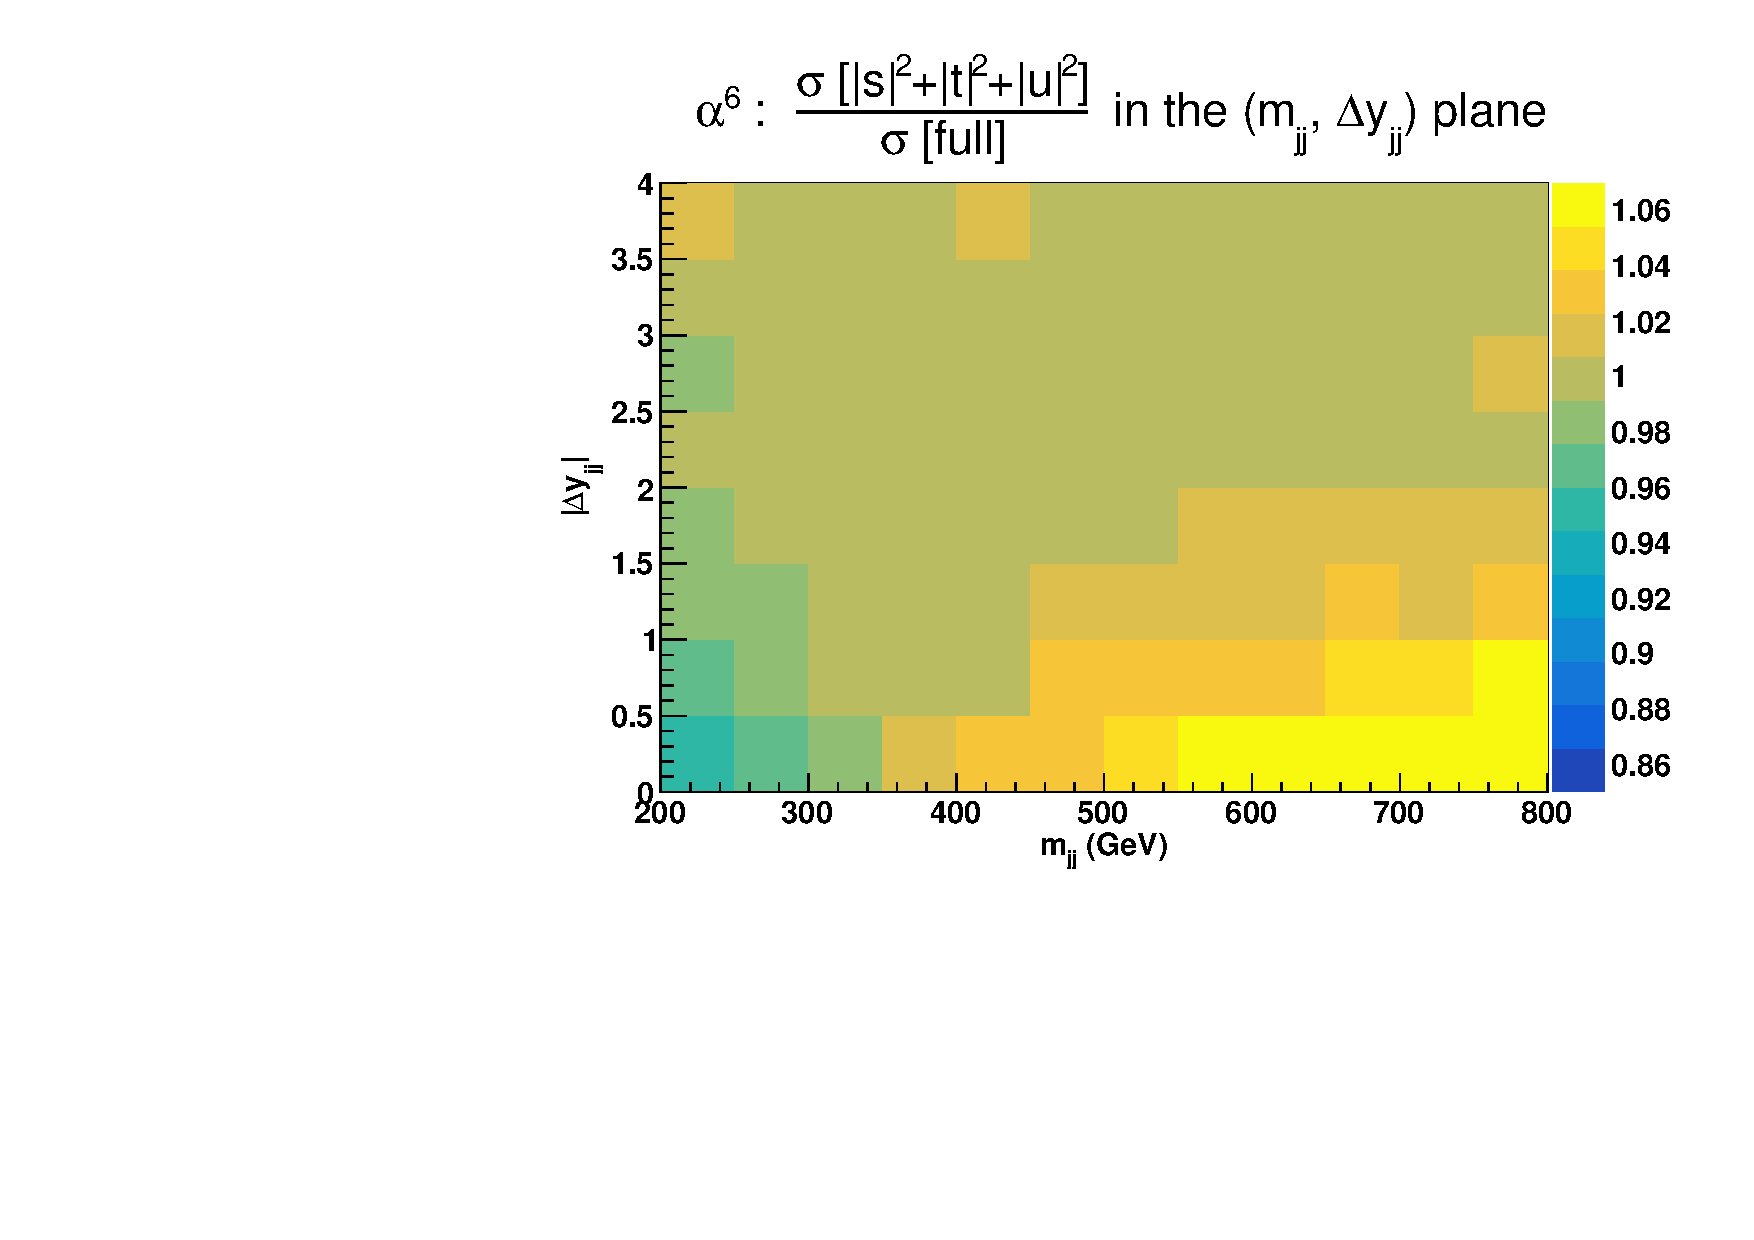
\includegraphics[scale=0.395]{figures/scanfigures/ratio_stu.pdf}
\caption{Cross sections (fb) per bin in the plan $\left(m_{\Pj\Pj}, \Delta y_{\Pj\Pj}\right)$ at order $\mathcal{O}(\alpha^6)$. 
Ratio of approximated squared amplitudes over the full matrix element. The approximated squared amplitudes are computed as $|\mathcal{A}|^2 \sim |t|^2 + |u|^2$ (left) and $|\mathcal{A}|^2 \sim |s|^2 + |t|^2 + |u|^2$ (right).}
\label{fig:ratio2d_LO}
\end{figure}

